% ClayBreeze project poster, built on the "stanford_beamer_poster" template
% by Sanha Cheong (https://github.com/sanhacheong/stanford_beamer_poster), MIT License —
% see LICENSE-template.txt in this folder. Unofficial template; not endorsed by Stanford
% University. The Stanford logos from the template are intentionally not used.
%
% Build (from this folder):  pdflatex ClayBreeze_Poster_Stanford.tex   (run twice)
% Output is copied to ../ClayBreeze_Poster_Stanford.pdf
\documentclass[final]{beamer}

% 36 x 24 in landscape, as in the template
\usepackage[orientation=landscape, scale=0.82, size=custom, height=60.96, width=91.44]{beamerposter}
\usetheme{confposter}
	\setbeamercolor{block title}{fg=cardinalred, bg=white}
	\setbeamercolor{block body}{fg=black, bg=white}
	\setbeamercolor{block alerted title}{fg=white, bg=cardinalred}
	\setbeamercolor{block alerted body}{fg=Black, bg=cloud}
\usepackage[font=small,labelfont=bf]{caption}

\usepackage{tabularx}
\usepackage{booktabs}
\usepackage[english]{babel}
\usepackage[utf8]{inputenc}
\usepackage{amsmath, amssymb}
\usepackage{graphicx}
\usepackage{fix-cm}
\usepackage{tikz}
\usetikzlibrary{arrows.meta}
\usepackage{textcomp}

\graphicspath{{../../media/photos/}{../../latex-shared/}}

% ClayBreeze accents alongside the template's Stanford palette
\definecolor{cbclay}{RGB}{184,80,31}
\definecolor{cbwater}{RGB}{26,111,148}
\definecolor{cbok}{RGB}{27,122,79}

% layout (template structure: separator + 4 columns)
\newlength{\sepwid}\setlength{\sepwid}{0.01\paperwidth}
\newlength{\firstcolwid}\setlength{\firstcolwid}{0.215\paperwidth}
\newlength{\secondcolwid}\setlength{\secondcolwid}{0.285\paperwidth}
\newlength{\thirdcolwid}\setlength{\thirdcolwid}{0.23\paperwidth}
\newlength{\lastcolwid}\setlength{\lastcolwid}{0.22\paperwidth}
\setlength{\topmargin}{-0.5in}

\addtobeamertemplate{block end}{}{\vspace*{0.4em}}
\addtobeamertemplate{block alerted end}{}{\vspace*{0.4em}}

\newcommand{\HUGE}{\fontsize{76}{84}\selectfont}
\newcommand{\emphg}[1]{{\color{paloalto}\textbf{#1}}}
\newcommand{\emphr}[1]{{\color{cardinalred}\textbf{#1}}}
\newcommand{\degC}{\,\textdegree C}
% photo tile: 960 x 1280 photo cropped to 6:5, caption below
\newcommand{\ph}[2]{\begin{minipage}[t]{0.32\linewidth}\centering\includegraphics[width=\linewidth,trim=0 240 0 240,clip]{#1}\\[0.2em]{\small #2}\end{minipage}}

% Headline: template layout, without the Stanford logos, rule sized to the paper
\setbeamertemplate{headline}{
 \leavevmode
  \begin{columns}
   \begin{column}{\linewidth}
    \vskip1.0cm
    \centering
    {\color{cardinalred}\HUGE\textbf{\inserttitle}}\\[0.6ex]
    {\color{coolgray}\Large\textbf{Makerspace \textperiodcentered\ Group 17 \textperiodcentered\ Tinkerers' Lab, Sanjivani University}}\\[1.0ex]
    {\Large\insertauthor}\\[0.7ex]
    {\large\insertinstitute}
    \vskip0.6cm
   \end{column}
  \end{columns}
 \begin{center}{\color{cardinalred}\rule{\dimexpr\paperwidth-2in\relax}{0.3cm}}\end{center}
 \vspace{0.1in}
}

\title{ClayBreeze --- A Sustainable Clay-Based Air-Cooling System}
\author{\textbf{Tanmay Nilesh Pendbhaje} (Leader) \textperiodcentered\ Harshal Kotame \textperiodcentered\ Vedant Khairnar \textperiodcentered\ Tanmay Mhaske}
\institute{Project Guide: \textbf{Dr.~Kiran Wakchaure} \textperiodcentered\ FY B.Tech Mechanical Engineering, Sanjivani University}
\date{}

\begin{document}
\begin{frame}[t]
\begin{columns}[t]

\begin{column}{\sepwid}\end{column}

% ---------------- column 1: problem, solution ----------------
\begin{column}{\firstcolwid}

\begin{alertblock}{Problem}
Summer heat in Indian homes, classrooms and workshops is a real problem, and affordable cooling is limited: India has one of the lowest levels of access to cooling in the world~[1].
\begin{itemize}
\item \textbf{Air conditioners:} expensive to buy and run, high electrical demand, refrigerants with climate impact --- out of reach for many households and schools.
\item \textbf{Honeycomb / cellulose pad coolers:} pads clog with scale and dust, degrade and need periodic replacement~[2]; plastic bodies.
\item \textbf{Grass (khus / wood-wool) pad coolers:} damp pads can harbour mould and bacteria, cause odour and attract insects, are combustible when dry and need frequent replacement~[4,5].
\end{itemize}
Pad coolers do cool --- the problem is the consumable pad and its upkeep.
\end{alertblock}

\begin{block}{Solution}
ClayBreeze replaces the pad with \emphr{30 porous, unglazed terracotta pots}, kept wet by recirculating water, with \emphg{smart ESP32 control}: each fan switched on temperature, the pump on humidity, with hysteresis.
\begin{itemize}
\item \textbf{Natural material:} locally made, reusable, biodegradable clay.
\item \textbf{No pad to replace:} the pots are the wetted medium; porous clay draws water through its walls~[3].
\item \textbf{Low power by design:} fans and pump run only when the readings call for them.
\end{itemize}
\textbf{Design aim:} low cost, low power, no pad replacement, eco-friendly. \emph{This is the aim, not a measured result.}
\end{block}

\end{column}

\begin{column}{\sepwid}\end{column}

% ---------------- column 2: working principle, CAD, build ----------------
\begin{column}{\secondcolwid}

\begin{block}{Working principle}
\centering
\resizebox{0.74\linewidth}{!}{% ClayBreeze working-principle schematic (side view), shared by the poster and the report.
% Conceptual — not measured. Coordinates follow the website SVG (x right, y down), 760 x 330 units.
% Use inside \resizebox{<width>}{!}{\input{.../schematic.tex}}.
\begin{tikzpicture}[x=1pt, y=-1pt, font=\sffamily\bfseries\fontsize{21}{24}\selectfont,
    air/.style={line width=3pt, -{Latex[length=14pt,width=12pt]}, black},
    bypass/.style={line width=2.2pt, dash pattern=on 9pt off 7pt, -{Latex[length=12pt,width=10pt]}, black!60},
    water/.style={line width=4pt, cbwater},
    lbl/.style={anchor=base west, inner sep=0pt}]
  % frame (main) and rear extension
  \draw[line width=3pt] (300,52) rectangle (380,266);
  \draw[line width=2.5pt, black!60] (380,52) rectangle (444,266);
  % pots on six rods
  \foreach \y in {74,108,142,176,210,244}
    \fill[cbclay, draw=white, line width=1.5pt] (310,\y) -- (332,\y-13) -- (348,\y-13) -- (361,\y) -- (348,\y+13) -- (332,\y+13) -- cycle;
  % fans
  \draw[line width=2pt, fill=black!8] (428,88) rectangle (439,148);
  \draw[line width=2pt, fill=black!8] (428,166) rectangle (439,226);
  % air path
  \draw[air] (600,118) -- (446,118);
  \draw[air] (600,196) -- (446,196);
  \draw[air] (424,118) .. controls (400,118) and (390,108) .. (364,108);
  \draw[air] (424,196) .. controls (400,196) and (390,176) .. (364,176);
  \draw[air] (300,108) -- (150,108);
  \draw[air] (300,176) -- (150,176);
  \draw[bypass] (424,92) .. controls (380,70) and (350,44) .. (300,44) .. controls (260,44) and (220,64) .. (150,64);
  \node[lbl] at (608,112) {Room air};
  \node[lbl] at (608,136) {in};
  \node[lbl] at (608,190) {Rear fans};
  \node[lbl] at (608,214) {blow forward};
  \node[lbl] at (4,100) {Out of};
  \node[lbl] at (4,124) {the front};
  \node[lbl] at (4,168) {More humid};
  \node[lbl, black!60] at (4,58) {Bypass};
  \node[anchor=base east, inner sep=0pt, black!60] at (272,264) {Front};
  \node[lbl, black!60] at (452,264) {Rear};
  % water path: tub -> pump -> tubing -> top of pots -> back to tub
  \draw[line width=3pt, cbwater, fill=cbwater!12] (250,276) rectangle (500,316);
  \draw[line width=3pt, cbwater, fill=white] (282,296) circle (13);
  \node[cbwater] at (282,296) {P};
  \draw[water, -{Latex[length=14pt,width=12pt]}] (282,283) -- (282,22) -- (330,22);
  \draw[water] (340,22) -- (372,22);
  \foreach \x in {318,340,362} \draw[cbwater, line width=2.5pt, dash pattern=on 4pt off 6pt] (\x,28) -- (\x,48);
  \draw[water, -{Latex[length=12pt,width=10pt]}] (371,262) -- (371,274);
  \node[lbl, cbwater] at (510,292) {Tub};
  \node[lbl, cbwater] at (510,314) {+ pump};
  \node[anchor=base east, inner sep=0pt, cbwater] at (272,226) {Tubing};
\end{tikzpicture}
}\\[0.3em]
\raggedright
\textbf{Air:} room air $\rightarrow$ rear fans $\rightarrow$ through \& around the wet pots $\rightarrow$ out of the front.\\
\textcolor{cbwater}{\textbf{Water:}} tub $\rightarrow$ pump $\rightarrow$ tubing $\rightarrow$ top of the pots $\rightarrow$ back to the tub.\\
{\small Evaporation from the wet clay takes heat from the air, which also becomes more humid~[2]. Conceptual --- not measured.}
\end{block}

\begin{block}{CAD (SolidWorks)}
\centering
\begin{minipage}[b]{0.76\linewidth}\centering
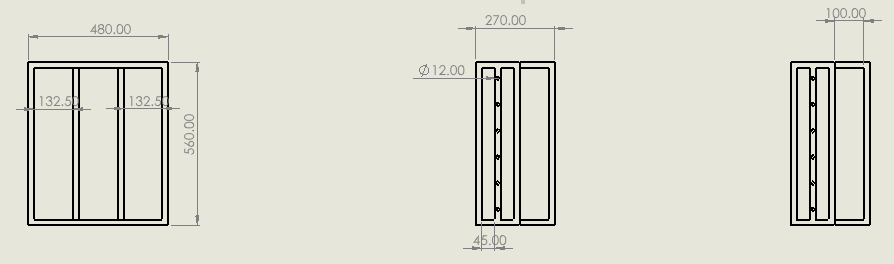
\includegraphics[width=\linewidth]{cad-drawing-dimensioned.png}\\[0.2em]
{\small Dimensioned drawing: 480 $\times$ 560 $\times$ 150\,mm frame, 270\,mm overall depth, $\varnothing$12\,mm rods}
\end{minipage}\hfill
\begin{minipage}[b]{0.19\linewidth}\centering
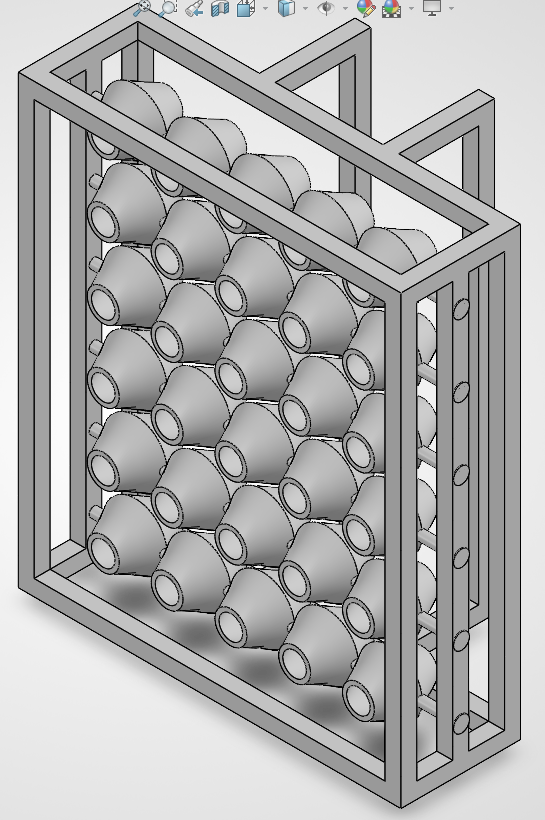
\includegraphics[width=\linewidth]{cad-assembly-isometric.png}\\[0.2em]
{\small Assembly}
\end{minipage}
\end{block}

\begin{block}{Build: fabrication to final assembly}
\centering
\ph{Frame_pipe_cutting_1.jpeg}{1 Pipe cutting}\hfill
\ph{Frame_Welded_1.jpeg}{2 Welded frame}\hfill
\ph{Frame_with_Rod_And_Exhaust_Fan_Colourd.jpeg}{3 Paint, rods, fans}\\[0.5em]
\ph{Frame_Completely_Assembled_Front_View.jpeg}{4 30 clay pots fitted}\hfill
\ph{Water_System_Tub_Front_Right_View.jpeg}{5 Final, in the water tub}\hfill
\ph{Water_System_Tub_Side_View.jpeg}{6 Side: fans, tubing, tub}
\end{block}

\end{column}

\begin{column}{\sepwid}\end{column}

% ---------------- column 3: specs, control logic, electronics ----------------
\begin{column}{\thirdcolwid}

\begin{block}{Key specifications}
\renewcommand{\arraystretch}{1.2}
\begin{tabularx}{\linewidth}{@{}l>{\raggedright\arraybackslash}X@{}}
\toprule
Frame & 480 $\times$ 560 $\times$ 150\,mm, 20\,mm square pipe, welded, painted \\
Front opening & 440 $\times$ 520\,mm \\
Overall depth & 270\,mm with rear fan mount \\
Rods & 6 $\times$ $\varnothing$12\,mm \\
Cooling medium & 30 unglazed terracotta pots (5 $\times$ 6) \\
Airflow & 2 exhaust fans, rear-mounted \\
Water & Tub, pump, tubing (recirculating) \\
Control & ESP32 + DHT11 + 3-ch relay \\
\bottomrule
\end{tabularx}
\end{block}

\begin{block}{Control logic (implemented, with hysteresis)}
\renewcommand{\arraystretch}{1.25}
\begin{tabularx}{\linewidth}{@{}>{\raggedright\arraybackslash}Xll@{}}
\toprule
\textbf{Output} & \textbf{ON} & \textbf{OFF} \\
\midrule
Fan 1 & \textcolor{cbok}{\textbf{$> 26$\degC}} & $\le 25$\degC \\
Fan 2 & \textcolor{cbok}{\textbf{$> 30$\degC}} & $\le 29$\degC \\
\textcolor{cbwater}{Water motor} & \textcolor{cbwater}{\textbf{RH $< 75$\,\%}} & \textcolor{cbwater}{RH $\ge 77$\,\%} \\
\bottomrule
\end{tabularx}\\[0.3em]
{\small Between the limits each output keeps its previous state, so the relays do not chatter. The pump stops in humid air, where evaporation has less cooling potential~[2].}
\end{block}

\begin{block}{Electronics}
\begin{itemize}
\item \textbf{ESP32} on a breadboard --- runs the logic
\item \textbf{DHT11} --- DATA on GPIO32 (7A), VCC from ESP32 3.3V
\item \textbf{3-channel relay} (active-low) --- IN1 GPIO25 Fan 1, IN2 GPIO26 Fan 2, IN3 GPIO27 water motor
\item \textbf{Firmware} --- \texttt{firmware/claybreeze\_controller}
\end{itemize}
\end{block}

\end{column}

\begin{column}{\sepwid}\end{column}

% ---------------- column 4: status, future, QR, references ----------------
\begin{column}{\lastcolwid}

\begin{alertblock}{Status}
\textcolor{cbok}{\textbf{\checkmark\ Build complete}} --- frame, 30 pots, fans, tub, pump, tubing.\\
\textcolor{cbok}{\textbf{\checkmark\ Control logic implemented}} --- running on the ESP32.\\[0.3em]
\textbf{Results:} no measured results are claimed.
\end{alertblock}

\begin{block}{Future scope}
\begin{itemize}
\item \textbf{Performance measurement:} inlet/outlet temperature and RH, airflow, water use and power against a dry-pot baseline.
\item \textbf{Data logging} of readings and relay states.
\item \textbf{IoT monitoring} over the ESP32's Wi-Fi.
\item \textbf{Improvements:} even water distribution, water-level sensing, fan guards, electronics in the laser-cut MDF enclosure, CAD updated to as-built.
\end{itemize}
\end{block}

\begin{block}{Live site, 3D model and docs}
\begin{minipage}[c]{0.36\linewidth}

\includegraphics[width=\linewidth]{qr-live-site.png}
\end{minipage}\hfill
\begin{minipage}[c]{0.6\linewidth}\raggedright
Scan for the interactive 3D model, photos and documentation.\\[0.4em]
{\small\color{cbwater}\texttt{tanmay-np.github.io/}\\\texttt{Claybreeze-Sustainable-}\\\texttt{Air-Cooling}}
\end{minipage}
\end{block}

\begin{block}{References}
\footnotesize\raggedright
[1] MoEFCC, Govt.\ of India. \emph{India Cooling Action Plan}, 2019.\par
[2] Watson et al. \emph{Fan and Pad Greenhouse Evaporative Cooling Systems}. Univ.\ of Florida IFAS, AE069.\par
[3] Laknizi et al. Direct evaporative cooling pad based on pottery material. \emph{Int.\ J.\ Sustainable Eng.} 14(1), 2021.\par
[4] Al-Sulaiman. Performance of local fibers in evaporative cooling. \emph{Energy Convers.\ Manag.} 43(16), 2002.\par
[5] Jain \& Hindoliya. New evaporative cooling pad materials. \emph{Sustain.\ Cities Soc.} 1(4), 2011.\par
\vspace{0.3em}
\textbf{Inspiration:} reporting on \emph{Project Vaayu}, a separate student initiative using clay kulhads for classroom cooling (Times of India, 2026). Not our project; its results are not ours.\par
\vspace{0.3em}
{\scriptsize Poster layout: stanford\_beamer\_poster template by S.~Cheong (MIT License); unofficial, not affiliated with Stanford University.}
\end{block}

\end{column}

\begin{column}{\sepwid}\end{column}

\end{columns}
\end{frame}
\end{document}
